%%%%%%%%%%%%%%%%%%%%%%%%%%%%%%%%%%%%%%%%%%%%%%%%%%%%%%%%%%%%%%%%%%%%%%%%%%%%%%%%%%%%%%%%%%%%%%%%%%%%%%%
%%													%%
%% 	BAKALÁŘSKÁ PRÁCE - Posun letecky měřených bodů po trajektorii v prostředí~QGIS 				%%
%% 				 Ondřej Pešek							%%
%%													%%
%% pro formátování využita šablona: http://geo3.fsv.cvut.cz/kurzy/mod/resource/view.php?id=775 	%%
%%													%%
%%%%%%%%%%%%%%%%%%%%%%%%%%%%%%%%%%%%%%%%%%%%%%%%%%%%%%%%%%%%%%%%%%%%%%%%%%%%%%%%%%%%%%%%%%%%%%%%%%%%%%% 

\documentclass[%
  12pt,         			% Velikost základního písma je 12 bodů
  a4paper,      			% Formát papíru je A4
  twoside,       			% Oboustranný tisk
  pdftex,				    % překlad bude proveden programem 'pdftex' do PDF
  draft
]{report}       			% Dokument třídy 'zpráva'
%

\usepackage[czech, english]{babel}	% použití češtiny, angličtiny
\usepackage[utf8]{inputenc}		% Kódování zdrojových souborů je UTF8

\usepackage[square,sort,comma,numbers]{natbib}

\usepackage{caption}
\usepackage{subcaption}
\captionsetup{font=small}
\usepackage{enumitem} 
\setlist{leftmargin=*} % bez odsazení

\makeatletter
\setlength{\@fptop}{0pt}
\setlength{\@fpbot}{0pt plus 1fil}
\makeatletter

\usepackage[dvips]{graphicx}   
\usepackage{color}
\usepackage{transparent}
\usepackage{wrapfig}
\usepackage{float} 

\usepackage{cmap}           
\usepackage[T1]{fontenc}    

\usepackage{textcomp}
\usepackage[compact]{titlesec}
\usepackage{amsmath}
\addtolength{\jot}{1em} 

\usepackage{chngcntr}
\counterwithout{footnote}{chapter}

\usepackage{acronym}

\usepackage[
    unicode,                
    breaklinks=true,        
    hypertexnames=false,
    colorlinks=true, % true for print version
    citecolor=black,
    filecolor=black,
    linkcolor=black,
    urlcolor=black
]{hyperref}         

\usepackage{url}
\usepackage{fancyhdr}

\usepackage[
  cvutstyle,          
  bachelor           
]{thesiscvut}


\newif\ifweb
\ifx\ifHtml\undefined % Mimo HTML.
    \webfalse
\else % V HTML.
    \webtrue
\fi 

\renewcommand{\figurename}{Obrázek}
\def\figurename{Obrázek}

%%%%%%%%%%%%%%%%%%%%%%%%%%%%%%%%%%%%%%%%%%%%%%%%%%%%%%%%%%%%%%%%%
%%%%%%%%%%% Definice informací o dokumentu  %%%%%%%%%%%%%%%%%%%%%
%%%%%%%%%%%%%%%%%%%%%%%%%%%%%%%%%%%%%%%%%%%%%%%%%%%%%%%%%%%%%%%%%

%% Název práce
\nazev{Posun letecky měřených bodů po trajektorii v~prostředí~QGIS}{}

%% Jméno a příjmení autora
\autor{Ondřej}{Pešek}

%% Jméno a příjmení vedoucího práce včetně titulů
\garant{Ing.~Martin~Landa,~Ph.D.}

%% Označení oboru studia
\oborstudia{Geodézie, kartografie a~geoinformatika}{}

%% Označení ústavu
\ustav{Katedra geomatiky}{}

%% Rok obhajoby
\rok{2016}

%Mesic obhajoby
\mesic{červen}

%% Místo obhajoby
\misto{Praha}

%% Abstrakt
\abstrakt 
{Cílem bakalářské práce je návrh softwarového nástroje umožňujícího posun letecky měřených bodů po trajektorii (tzv.~leveling leteckých dat). Takový nástroj je třeba z~toho důvodu, že přístroj při leteckých měřeních zapisuje souřadnice s~určitým zpožděním. V~praktické části práce se objevuje jeho implementace jako tzv.~zásuvného modulu do prostředí open source projektu QGIS s~využitím grafického frameworku Qt. }%
{The object of bachelor thesis is creation of software tool for moving aerial data by their trajectory (aerial data leveling). The reason for this tool is that the instrument for aerial data surveying is recording data with some delay. In practical part of bachelor thesis is implementation of this tool as plugin into open source project QGIS using graphical framework Qt. 
 }

%% Klíčová slova
\klicovaslova
{GIS, Quantum~GIS, zásuvný~modul, python, leveling}%
{GIS, Quantum~GIS, plugin, python, leveling}

%%%%%%%%%%%%%%%%%%%%%%%%%%%%%%%%%%%%%%%%%%%%%%%%%%%%%%%%%%%%%%%%%%%%%%%%

%%%%%%%%%%%%%%%%%%%%%%%%%%%%%%%%%%%%%%%%%%%%%%%%%%%%%%%%%%%%%%%%%%%%%%%%
%% Nastavení polí ve Vlastnostech dokumentu PDF
%%%%%%%%%%%%%%%%%%%%%%%%%%%%%%%%%%%%%%%%%%%%%%%%%%%%%%%%%%%%%%%%%%%%%%%%
\nastavenipdf
%%%%%%%%%%%%%%%%%%%%%%%%%%%%%%%%%%%%%%%%%%%%%%%%%%%%%%%%%%%%%%%%%%%%%%%

%%% Začátek dokumentu
\begin{document}

\catcode`\-=12  % pro vypnuti aktivniho znaku '-' pouzivaneho napr. v \cline 

% aktivace záhlaví
\zahlavi

% předefinování vzhledu záhlaví
\renewcommand{\chaptermark}[1]{%
	\markboth{\MakeUppercase
	{%
	\thechapter.%
	\ #1}}{}}

% Vysázení přebalu práce
%\vytvorobalku

% Vysázení titulní stránky práce
\vytvortitulku

% Vysázení listu zadani
\stranka{}%
	{\sffamily\Huge\centering\ ZDE VLOŽIT LIST ZADÁNÍ}%
	{\sffamily\centering Z~důvodu správného číslování stránek}

% Vysázení stránky s abstraktem
\vytvorabstrakt

% Vysázení prohlaseni o samostatnosti
\vytvorprohlaseni

% Vysázení poděkování
\stranka{%nahore
       }{%uprostred
       }{%dole
       \sffamily
	\begin{flushleft}
		\large
		\MakeUppercase{Poděkování}
	\end{flushleft}
	\vspace{1em}
		%\noindent
	\par\hspace{2ex}
	{Chtěl bych poděkovat vedoucímu práce, Ing.~Martinu Landovi,~PhD., za připomínky a~pomoc při zpracování této práce. }
}

% Vysázení obsahu
\obsah

% Vysázení seznamu obrázků
\seznamobrazku

% Vysázení seznamu tabulek
\seznamtabulek

% jednotlivé kapitoly
\chapter{Úvod}
\label{1-uvod}

*********************************************************************
CHYBÍ PRVNÍ ČÁST - NEVÍM, ZDA POUŽÍVAT SLOVO LEVELING + DOPLNIT ZDROJE A CITACE
*********************************************************************

Zájem o~vývoj takového zásuvného modulu pochází od Státního ústavu radiační ochrany (\zk{SÚRO}).
\zk{SÚRO} se zabývá mimo jiné vyhledáváním lokalit se zvýšenou koncentrací radonu a~vedením centrální
databáze takových míst, poskytováním konzultací, prováděním laboratorních expertíz a~hodnocením
radiační ochrany v~oblasti lékařského ozáření. 

Ústav se rovněž angažuje v~oblasti výzkumných projektů, například „výzkum pokročilých metod detekce,
stanovení a~následného zvládnutí radioaktivní kontaminace s~cílem modernizovat odpovídající části
systému zajištění ochrany obyvatel a~vybraných kritických infrastruktur ČR v~souvislosti
s~radiologickým útokem nebo velkou radiologickou havárií“ nebo „testování nových systémů
hromadného měření radiojódu ve štítné žláze po havárii jaderně energetického zařízení“. 

Velkou část činností \zk{SÚRO} tvoří též terénní měření a~následné zpracování
těchto dat v~prostředí QGIS. 



\chapter{Teoretický základ}
\label{2-teorie}

%%% ML: vyplynuti posunu, v dalsi vete "body"
Tato kapitola si klade za cíl seznámit čtenáře s~teoretickými základy měření radioaktivity, z~nichž
plyne potřeba posunu měřených bodů. Dále pak načrtne způsoby, kterými bude možno body posouvat, a~popíše
nejdůležitější problémy, s~nimiž se při takovém posunu lze setkat. 

%%% ML: pridat poznamku o zdroji 

\section{Scintilační spektrometrie}
\label{spektrometrie}

V~kapitole o~scintilační spektrometrii bylo vycházeno z~\citep{spektrometrie}. 

Ježto lidský subjekt není sám o~sobě schopen detekovat ionizující záření, je třeba si vypomoci příslušnou
technikou, tedy přístroji, detektory ionizujícího záření. Tako\-vých přístrojů existuje velké
a neustále se zvětšující množství. 

Obecně se detektory dělí buď podle průběhu detekce v závislosti na čase (kumulativní a~kontinuální),
nebo podle principu detekce (materiálové, fotografické a~pro nás nejdůležitější elektronické). 

  \begin{figure}[H]
   \centering
	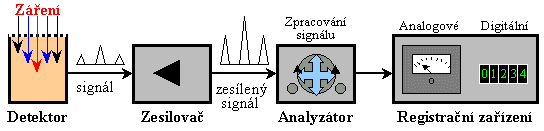
\includegraphics{./pictures/elektronicky-detektor.png}
	\caption[Základní schéma elektronického detektoru záření]{Základní schéma elektronického
	detektoru záření
	(zdroj: \cite{spektrometrie})}
      \label{fig:elektronicky-detektor}
  \end{figure}

Běžný elektronický detektor ionizujícího záření se skládá ze dvou hlavních bloků - z~detektorové
a~analyzační části. V~detektoru dochází k~transformaci ionizačního záření na měřitelné
elektronické impulsy. Takové impulsy bývají zesilovány buď už v~detektoru, nebo v~následujícím
zesilovači; často se užívá kombinace obého. Signál zesílený na měřitelnou odezvu poté putuje do
analyzátoru, který uživateli předává informace buď analogovou formou (například výchylka ručičky),
nebo formou di\-gitální (číselný ukazatel, zápis do souboru v~počítači). 

Následující podkapitoly představí přístroj a~metodu současně velice využívané,
totiž scintilační spektrometry. Scintilační spektrometry patří do elektronických detektorů
a~pro naši práci je důležité, že se objevují též v terénním měření \zk{SÚRO}. 

  \begin{figure}[H]
   \centering
	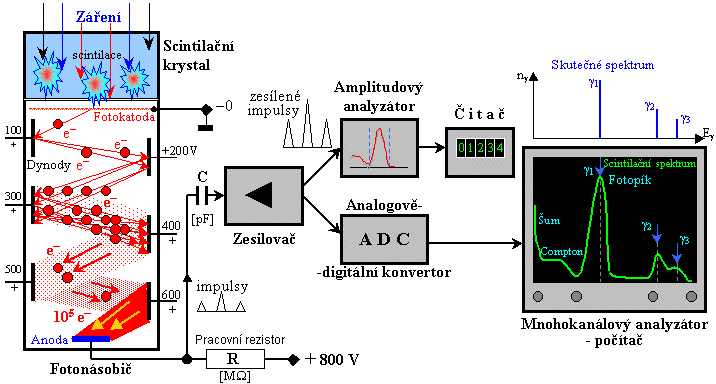
\includegraphics[scale=0.75]{./pictures/scintilacni-detektor.png}
	\caption[Obecné schéma scintilačního detektoru]{Obecné schéma scintilačního detektoru
	(zdroj: \cite{spektrometrie})}
      \label{fig:scintilacni-detektor}
  \end{figure}

\subsection{Detektorová část}
\label{detektor}

Ve scintilačních detektorech zachycuje ionizační záření takzvaná scintilační sonda.
%%% ML: Ta *se* sestava?
Ta se skládá ze scintilačního krystalu a~fotonásobiče umístěných ve světlotěsném pou\-zdře.
Pouzdro nejen že zabraňuje vniku nadbytečného světla do detekční jednotky, ale také stíní
vnější magnetické pole, které by mohlo ovlivňovat správnou funkci fotonásobiče. 

Obecná práce scintilačního detektoru spočívá v~tom, že detekuje-li nějaké ionizační záření, dochází ve
scintilačním krystalu ke světelným zábleskům. Emise fotonů jsou přímo úměrné absorbovanému záření.
Pomocí fotoelektrického jevu je ve vstup\-ní fotokatodě fotonásobiče převedeno fotonové kvantum na kvantum
elektronové, načež uvnitř fotonásobiče dojde k zněkolikanásobení elektronů. 

\subsubsection{Scintilační krystal}
\label{krystal}

Existují látky, takzvané scintilátory, které na pohlcení kvant ionizujícího záření reagují
scintilacemi (z~latinského scintilla~-~jiskra\footnote{zdroj: FÜRST, Kamil a MEISSNER, Josef:
\textit{Slovník latinsko-český a česko-latinský}, Praha: Nakladatelé Kvasnička a Hampl, 1941}, scintilace
tedy představují světel\-né záblesky).
Byť se mohou objevovat i~scintilátory kapalné či plynné, zde se budeme zabývat scintilátory
nejběžněji užívanými - krystaly. 

Krystaly bývají planárního válcového tvaru, případně pro speciálnější účely (vy\-soko\-energetická záření,
detekce měkkého záření gama) velkoobjemové, studnové či tenké. V~současné době jsou krystaly
nejčastěji vyráběny z~jodidu sodného aktivovaného thaliem (\textit{NaI(Tl)}), dříve se též
používal sirník zinečnatý aktivovaný stříbrem nebo kyanid platino-barnatý. 

Pokud bychom scintilátor jen přivařili ke vstupnímu okénku fotonásobiče, dochá\-zelo by
ve vzduchové vrstvě mezi výstupním okén\-kem scintilátoru a vstupním okén\-kem fotonásobiče k~nechtěné
ztrátě fotonů. Tento prostor tedy bývá zaplňován látkou s~vysokou světelnou vodivostí, například
silikonovou vazelínou. V~případě většího průzvu bývají oba elementy spojeny světlovodičem či
optickými vlákny. 

\subsubsection{Fotonásobič}
\label{fotonasobic}

Fotonásobič představuje optoelektronickou součástku, která na základě fotoelektrického jevu
převádí světelný tok na elektrické signály. Jeho výhoda tkví ve vysoké citlivosti způsobené
několikanásobným zvětšením počtu elektronů pomocí dynod, pročež lze i~z~jediného fotonu
vyprodukovat dobře detekovatelný elektronický impuls. Fotonásobič tak navzdory svému názvu nenásobí
fotony, nýbrž elektrony vyvolané prvotním dopadem fotonů na fotokatodu. 

Vstupním elementem fotonásobiče je tedy fotokatoda. Jedná se o~tenkou vrstvu napařenou na
vstupním okénku, tvořenou zejména antimonidy alkalických prvků (nejčastěji cesia a antimonu),
%%% ML: ana?
ana převádí dopadající fotony fotoelektrickým jevem na elektrony.
Tenkost tvoří důležitou součást její výroby; v~opačném případě by mohlo docházet k~pohlcování
emitovaných elektronů v~materiálu fotokatody. 

Za fotokatodou (mezi fotokatodou a~první dynodou) se může nacházet kladně nabitá mřížka.
Její kladné napětí udává emitovaným elektronům vyšší rychlost a~usměrňuje je na první z~dynod. 

Následně tyto vyloučené elektrony násobí sekundární emise na dynodách. Dy\-nody představují soustavu
zvláštních elektrod, kde se na každou následující přivádí vyšší (zpravidla o~100~V nebo
%%% Na tomto principu funcuje i ?
%%%%%% OP: Na tomto principu fungují veškeré fotonásobiče; nevím tedy, 
%%%%%%     zda mám dohledávat i jiná zařízení, jsou-li
dvojnásobné) kladné napětí, pročež přitahují emitované elektrony. Tento systém funguje
jako elektronový zesilovač. Každá z~dynod pracuje tím způsobem, že po nárazu jednoho elektronu emituje
další elektrony. Mezi počtem vyražených elektronů a~kinetickou energií dopadajícího elektronu
platí přímá úměra. Obvykle se počet elektronů na každé dynodě zdvojnásobí. Několikerým
%%% ML: mrdani - poznamka pod carou ;-)
mrdáním\footnote{Slovo \textit{mrdati} zde není užito v~dnešním zdevalvovaném usu, alebrž ve svém prvotním
významu - tedy rychle se pohybovati, vrtěti, kroutiti. Označuje ale také rychlý pohyb na základě cizího
přičinění či pohyb a~odrážení vrženého tělesa. Takovýto význam zůstal zřetelný i~ve slovenském
\textit{mrdnúť}. Současná čeština nemá výstižnějšího výrazu. Viz příklad \textit{Byť jí prstem
po ústech mrdl, uzřel by...} \newline zdroj: KOTT, František Štěpán: \textit{Česko-německý slovník zvláště
grammaticko-fraseologický}, Praha: Nákladem J. Kolář/František Šimáček, 1878} elektronů dojde k~jejich
množení geometrickou řadou. Dynody mívají zpravidla
zakřivený tvar (vhodnější pro fokusaci elektronů na další dynodu). 

Posledním prvkem pak jest anoda - sběrná elektroda s~nejvyšším napětím, z~níž už přes pracovní
odpor \textit{R} pokračuje výstupní signál do zesilovače, případně přímo do analyzační části. 

  \begin{figure}[H]
   \centering
	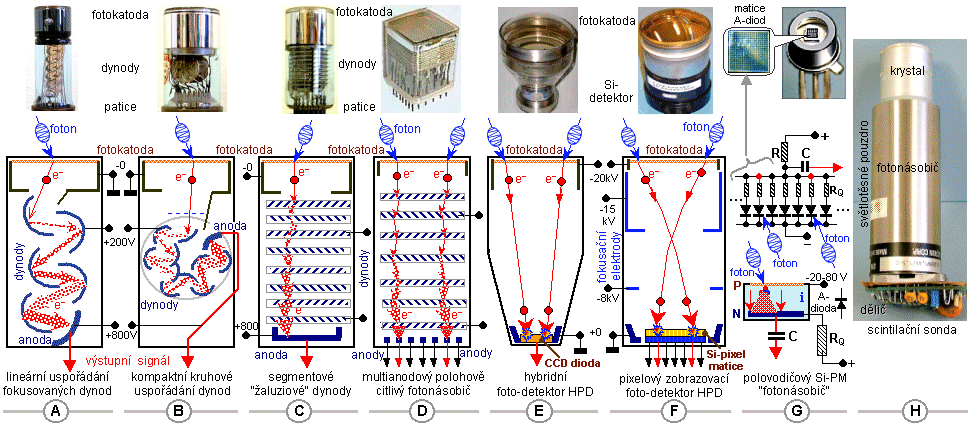
\includegraphics[scale=0.5]{./pictures/fotonasobice.png}
	\caption[Různá uspořádání fotonásobičů]{Různá uspořádání fotonásobičů
	(zdroj: \cite{spektrometrie})}
      \label{fig:fotonasobice}
  \end{figure}

\subsection{Analyzační část}
\label{analyzator}

Zesílené elektrické signály je třeba dále analyzovat. Existují dva druhy analyzátorů,
které prezentují v~obrázku \ref{fig:scintilacni-detektor} dvě paralelní větve. 

V~případě amplitudového analyzátoru se měří počet impulsů s~amplitudou mezi nastavenými
diskriminačními hladinami. Diskriminační hodnoty představují amplitudové infimum a~supremum.
Amplitudy ležící mimo toto rozmezí nebudou k~čítači propuštěny. Tím se částečně
eliminují chyby a~temný proud - proud protékající fotonásobičem i~bez ozáření fotokatody.
%%% ML: pik (tzv.)
Územ bývá nastavit toto rozmezí tak, aby obsahovalo takzvaný fotopík (\textit{pík totální absorpce})
záření měřeného radionuklidu. Impulsy zkrácené o~přebytečné hodnoty následně vstoupí již do čítače
impulsů. 

Spektrometrická analýza vyžaduje transformaci impulsů na bitové informace; k~té dochází
v~analogově-digitálním převodníku. V~paměti počítače se každé amplitudě záření gama
střádacím algoritmem přidělí buňka. Při detekci takového kvanta se její hodnota zvyšuje o~1.
Takovým postupem získáme scintilační spektrum, jehož grafické
znázornění je na obrázku \ref{fig:scintilacni-detektor}. 

\section{Sběr souřadnic a potřeba posunu}
\label{potreba posunu}

%%% ML: sber mereni
Sběr dat probíhá letecky. Scintilační spektrometr je uložen ve vrtulníku, který přelétá nad zkoumaným
územím; při přeletu se v~spektrometru registrují hodnoty záření. Tato data jsou registrována v~podstatě
neustále, ale zapisují se až po jistém časovém úseku (běžně po vteřině) jako průměr hodnot za onen
časový úsek měřených. V~okamžiku zápisu hodnot radionuklidů se rovněž tak zapisují zeměpisné souřadnice
(a~další parametry). Ty se však nijak neprůměrují, zapisují se momentální hodnoty. 

Z~popsaného plyne, že se registrované zeměpisné souřadnice od souřadnic geometrického průměru snímaného
pole liší; jedná se o~souřadnice začátku nebo konce měření v~dané epoše (záleží na použitém přístroji).
Vzniká tedy potřeba korekce zpoždění/předbíhání záznamu souřadnic oproti měřeným hodnotám. 

\section{Posun}
\label{posun}

Bohužel není k~dispozici záznam výšek vrtulníku během letu, ani přesný záznam jeho rychlosti, tudíž
není možnost dokonalé souřadnicové korekce, různými algoritmy se ale ideální hodnotě můžeme alespoň
přiblížit. Zásuvný modul umožňuje tři základní posuny měřených dat. 

Nejjednodušším způsobem je posun o~hodnoty. Hodnotě každého bodu přiřadíme souřadnice bodu
předcházejícího či následujícího (s~libovolným krokem). Takový posun ovšem nijak neposouvá jednotlivé
body, alebrž jen vzájemně vyměňuje jejich souřadnice. Před vývojem zásuvného modulu byl však tento
\textit{posun} tím zdaleka nejvyužívanějším, téměř bezkonkurenčně, pro svou jednoduchost - stačilo
posunout sloupce s potřebnými daty o~zamýšlený počet hodnot. 

  \begin{figure}[H]
   \centering
	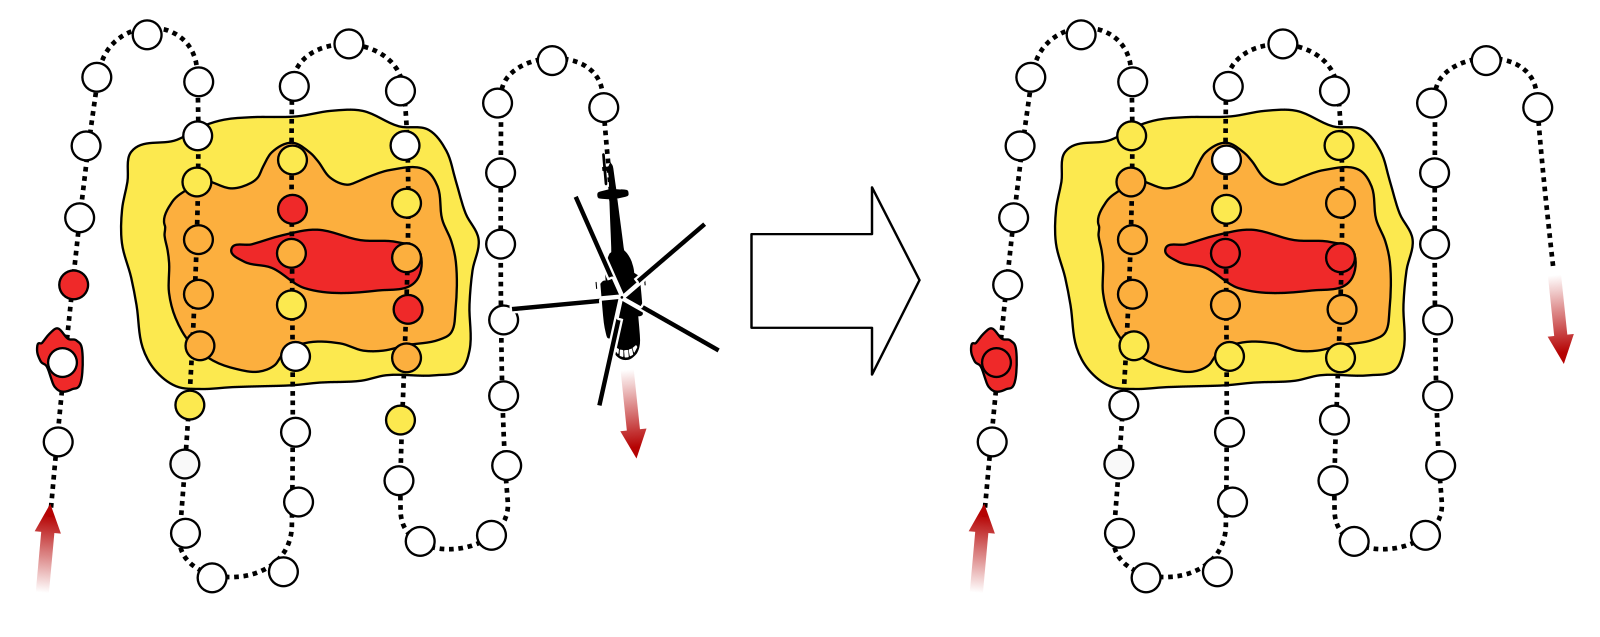
\includegraphics[scale=0.2]{./pictures/posun.png}
	\caption[Posun dat o 1 bod]{Posun dat o 1 bod
	(zdroj: HELEBRANT, Jan a GRYC, Lubomír: \textit{GPS position lag correction} [interní dokument
	SÚRO, v.v.i.])}
      \label{fig:posun}
  \end{figure}

Nápaditěji působí posun o~konstantní vzdálenost. Uživatel dostane možnost posunout všechny body
po trajektorii letu o~jím volenou vzdálenost. Tento princip představuje již skutečný, realitu lépe
vystihující posun. V~ideálním případě popsaném na následujících obrázcích by posun o~14 metrů přesunul
body na jejich náležité místo. 

  \begin{figure}[H]
   \centering
	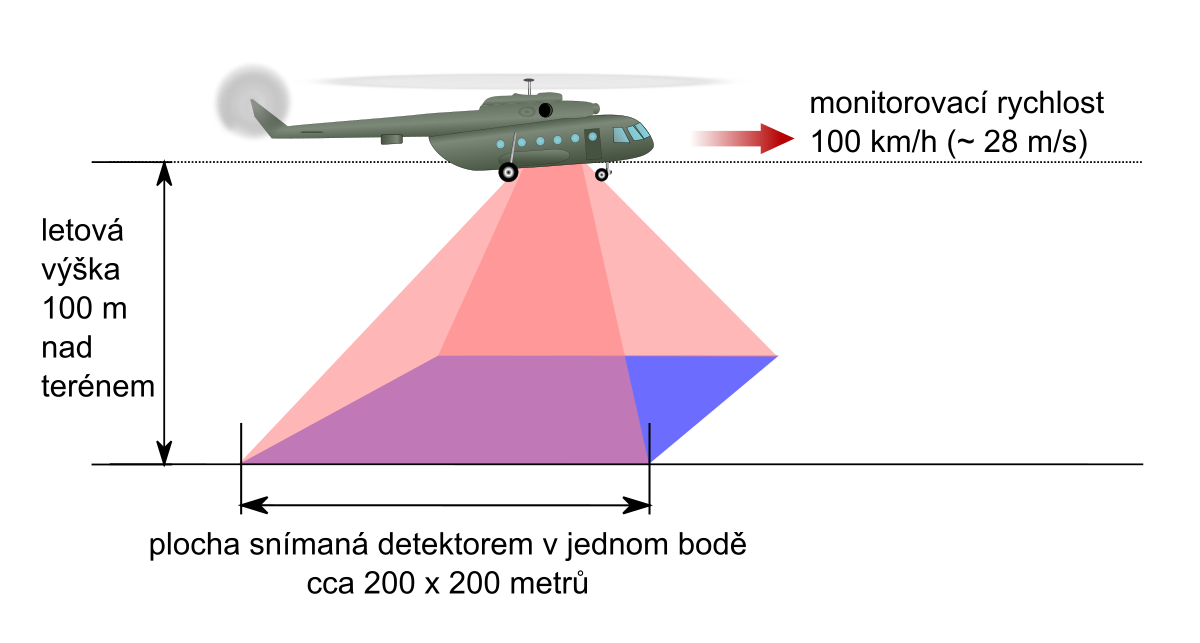
\includegraphics[scale=0.3]{./pictures/snimani.png}
	\caption[Princip měření]{Princip měření
	(zdroj: HELEBRANT, Jan a GRYC, Lubomír: \textit{GPS position lag correction} [interní dokument
	SÚRO, v.v.i.])}
      \label{fig:mereni}
  \end{figure}
  
  \begin{figure}[H]
   \centering
	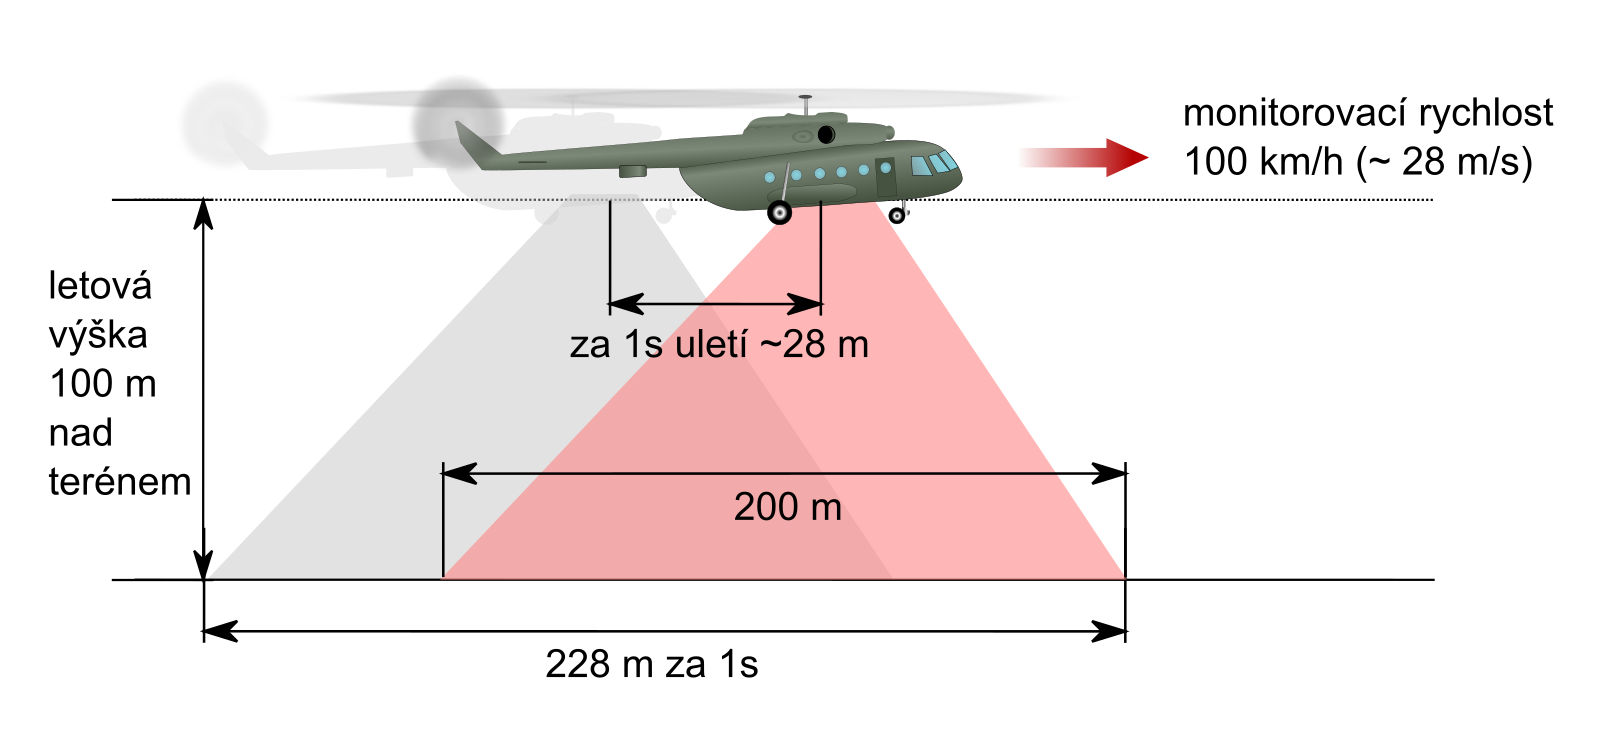
\includegraphics[scale=0.25]{./pictures/snimani-detail.png}
	\caption[Profilové schéma měření]{Profilové schéma měření
	(zdroj: HELEBRANT, Jan a GRYC, Lubomír: \textit{GPS position lag correction} [interní dokument
	SÚRO, v.v.i.])}
      \label{fig:mereni-profil}
  \end{figure}
  
Skutečnosti nejvěrněji odpovídá posun o~sekundy. V~dřeni se jedná o~posun o~vzdálenost, ale tentokráte
nikoli konstantní. 

Ze známých zeměpisných souřadnic se mezi každou dvojicí bodů vypočte vzdále\-nost. Neboť známe pro každý
z~bodů časovou značku, lehce (rozdíl dvou hodnot) vypočteme dobu, za niž vrtulník tuto vzdálenost urazil.
Tím získáme veškeré potřebné veličiny pro výpočet rychlosti mezi dvěma body. Následuje postup opačný:
Na zá\-kladě uživatelem zadané doby, o~niž se mají body posunout, se vypočte vzdálenost, kterou by
vrtulník za danou dobu urazil. Vztáhneme-li tuto vzdálenost opět na trajektorii pohybu, obdržíme
souřadnice posunutého bodu. 

\section{Problémy}
\label{problemy}

%%% ML: softwaroveho nastroje
%%% ML: dvakrat slovo "mhoho" v jedne vete
Při tvorbě softwarového nástroje, který by jmenované operace umožňoval, může dojít k~mnoha nepříjemnostem
a~problémům, s~nimiž je třeba se vypořádat. Jmenujme alespoň dva nejdůležitější: 

\subsection{Elipsoid}
\label{elipsoid}

Ačkoli různé typy spektrometrů produkují odlišné výstupy a~některé mohou obsahovat i~zeměpisné souřadnice
na jiném referenčním tělese, zpravidla obsahují (také) souřadnice na elipsoidu \zk{WGS84}. 

%%% ML: diafragma (...)
Přítomnost elipsoidických souřadnic namísto rovinných vnáší do výpočtu záludnou překážku, na niž musí
tvůrce algoritmu dbát zvýšeného zřetele. Od výpočtů na referenční kouli (nerci v~rovině) se
zásadně liší nejen délka, ale také azimut. Nejkratší spojnice (takzvaná geodetická křivka), která
reprezentuje také trajektorii mezi sousedními body, pak samozřejmě
v~rovinném zobrazení nemá tvar úsečky. Majoritu těchto problémů vyřešíme užitím první základní
geodetické úlohy na elipsoidu. 

\subsection{První geodetická úloha}
\label{prvnigu}

První geodetická úloha představuje hledání (výpočet) parametrů bodu na konci křivky, v~případě
%%% ML: softwarove / programoveho nastroje
představovaného softwarového nástroje na referenčním elipsoidu. Zná\-mými parametry jsou souřadnice
počátečního bodu křivky a~její azimut v~tomto bodě. Hledanými parametry zeměpisné souřadnice koncového
bodu. Zkoumaná křivka reprezentuje geodetickou křivku. 

Základní geodetické úlohy se dají řešit nejedním způsobem a~v~minulosti vždy znamenaly mnohé potíže
a~dlouhé výpočty. S~rozvojem informačních technologií došlo k~značnému urychlení výpočtu.
Prezentovaný princip vychází z~principu popisovaného v~\cite{vyssigeodezie} a~vycházejícího
z~postupu Ing.~Jana Douši. 

Postup spočívá v~rozdělení křivky na integrační kroky. Křivku, resp.~její úsek~\textit{h}
aproximujeme polynomem čtvrtého stupně, takzvanou Runge-Kuttovou metodou řádu~4. Potíž spočívá v~tom,
na kolik úseků máme danou křivku rozdělit. Přesnost totiž ovlivňuje nejen délka křivky, ale také její
poloha na elipsoidu. 

Daný problém řeší postupné iterace. Křivka se postupně půlí, následně se půlí její poloviny atd. (jde
tedy o~\textit{1/n}~násobky původní délky, kde \textit{n} představuje mocniny dvou), než dosáhneme
požadované přesnosti. Ta je kontrolována pomocí podmínky cyklu: Pokud se od sebe všechny vypočtené
atributy koncového bodu křivky ve dvou po sobě jdoucích iteracích liší o~hodnotu menší než danou
(v našem případě 0.0000000001~úhlového stupně), jsou poslední vypočtené atributy brány jako výsledné. 


  \begin{figure}[H]
   \centering
	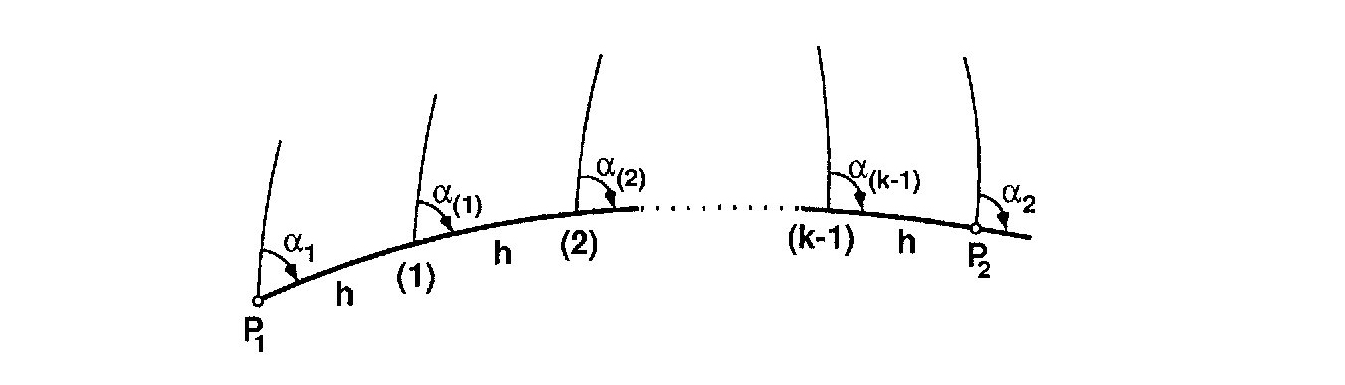
\includegraphics[scale=0.4]{./pictures/prvnigu-integrace.png}
	\caption[Integrační kroky v první geodetické úloze]{Integrační kroky v první geodetické úloze
	(zdroj: \cite{vyssigeodezie})}
      \label{fig:prvnigu-integrace}
  \end{figure}






\chapter{Použité technologie}
\label{3-technologie}

Třetí kapitola se zabývá užitými technologiemi, stručně představuje jejich historii a~zaměření.
Podrobnější informace o~jednotlivých projektech lze nalézt na oficiálních internetových stránkách. 


\section{Python}
\label{python}

  \begin{figure}[H]
   \centering
	
\includegraphics[scale=0.5]{./pictures/python-logo-master-v3-TM.png}
	\caption[Python logo]{Python logo 
      (zdroj: \url{https://www.python.org/static/community_logos/python-logo-master-v3-TM.png})}
      \label{fig:python}
  \end{figure}

Python je open-source multiplatformní programovací interpretovaný jazyk pojme\-novaný podle
kultovního britského komediálního seriálu Monty Pythonův létající cirkus. Momentálně se
vyvíjejí verze třetí řady (3.X). 

První verzi vydanou roku 1991 navrhl nizozemský programátor Guido van~Rossum za užití kódu
mnoha dalších programátorů. Silnou inspiraci van~Rossum našel v~jazyku ABC. Odtud také plyne
přívětivost jazyka, pro niž je často vyučován a~doporučován jako ideální pro rychlý
(a~přesto kvalitní) vývoj aplikací. 

Zásadní byl pro vývoj rok~2001, kdy vznikla nezisková organizace Python Software
Foundation (\zk{PSF}). \zk{PSF} zaštiťuje další vývoj Pythonu, vlastní jeho
\textit{intelektuální jmění} a~pořádá a~podporuje konference ohledně Pythonu. Sám van~Rossum bývá
pro svůj dohled a~svou neomezenou možnost zasahovat do vývoje nazýván \textit{benevolentní doživotní
diktátor}, španělská inkvizice jazyka Python. 

Python se na první pohled vyznačuje odsazováním kódu. Toho se ve většině jazyků používá jen jako
pomůcky pro přehlednost, v~Pythonu je však odsazování povinné. 

Mezi další specifikace jazyka patří například: 
\begin{itemize}

	\item Chování funkce: Ta se do svého zavolání uchovává jako objekt. 
	
	\item Proměnné: Není třeba deklarovat jejich typ. To může ušetřit značné množství práce
	v~psaní kódu, ale je třeba si na tuto vlastnost dát pozor (celé číslo dělené celým číslem je
	vždy celé číslo, i kdyby správným výsledkem mělo být číslo desetinné). 
	
	\item Proměnné uvnitř objektu: Není třeba je udávat při vytváření objektu. Lze je založit později. 
	
	\item Dokončení zápisu: V~interaktivním režimu provádím dokončení zápisu prázdným řádkem. 
	
	\item Kompilace: Python si automaticky kompiluje moduly do souborů \textit{.pyc}. Zkompilovaný
	modul je platformně nezávislý. 

\end{itemize}


\section{QGIS}
\label{qgis}

  \begin{figure}[H]
    \centering
      
\includegraphics[width=120pt]{./pictures/qgis.png}
      \caption[QGIS logo]{QGIS logo 
      (zdroj: \href{https://commons.wikimedia.org/wiki/File:QGIS\_logo.svg}{Wikimedia Commons})}
      \label{fig:qgis}
  \end{figure}

QGIS (zkratka dříve užívaného názvu Quantum~GIS) představuje na poli geogra\-fic\-kých informačních systémů (\zk{GIS}) open-source alternativu ke komerčním geografickým informačním systémům typu~ArcGIS. 

Na začátku 21.~století už byly geografické informační systémy běžnou praxí. Zrodila se tedy potřeba volby svobodného multiplatformního systému s~širokou podporou formátů geodat. Roku 2002 začal Quantum~GIS vyvíjet Gary~Sherman, k~němuž se později připojovalo čím dál více dobrovolníků. Časem projekt zaštítilo též Open Source Geospatial Foundation (\zk{OSGeo})~–~organizace pro podporu a~vývoj otevřených geoinformačních technologií a dat vzniklá roku~2006. Verze~1.0 byla uveřejněna v~lednu~2009. 

První verze systému QGIS byly pojmenovávány podle psů, později se přešlo na jména měsíců Jupiteru a~Saturnu. Momentálně nesou nejnovější verze názvy měst. 
QGIS se ve svém zaměření příliš neliší od běžných geografických informačních systémů. Uživatel v~něm má možnost prohlížení, zpracování, tvorby a~editace geodat, nad nimiž může provádět například SQL~dotazy. Data v~prostředí QGIS mohou být jak rastrová, tak také vektorová. Co se funkcionality týče, běžnému uživateli dostačuje, ale možností komerčních gigantů typu ArcGIS nedosahuje. 

Síla QGIS vedle volnosti užití tkví především ve značném množství veřejně přístupných zásuvných modulů~–~tzv.~pluginů. Ty byly zprvu psány především v~jazyku C++ (stejně jako základní tělo programu), nyní se čím dál častěji přechází k~jazyku Python, přičemž především pro grafické uživatelské rozhraní se využívá Qt~knihoven. 



\section{Qt Project}
\label{qt}

  \begin{figure}[H]
    \centering
      
\includegraphics[width=120pt]{./pictures/qt.png}
      \caption[Qt logo]{Qt logo 
      (zdroj: \url{http://d3hp9ud7yvwzy0.cloudfront.net/wp-content/uploads/2015/02/Qt-logo-medium.png})}
      \label{fig:qt}
  \end{figure}

Qt představuje uživatelsky přívětivé multiplatformní vývojové prostředí s~důrazem na grafické
uživatelské rozhraní (\zk{GUI}). 

Vývoj Qt započali na úsvitu devadesátých let dva programátoři - Haavard Nord a~Eirik
Chambe-Eng. Původně dali své společnosti jméno Quasar technologies, ale brzy společnost
přejmenovali na Trolltech. Pod touto hlavičkou působili až do roku~2008, kdy firmu odkoupila
Nokia. V letech 2011 a~2012 pak probíhal další přesun, tentokráte pod podnik Digia. Digia
nadále spolupracuje s~Qt~Company. 

Qt není programovacím jazykem. Qt je framework psaný v~C++, umožňující ale práci i~v~dalších jazycích
včetně jazyka python (PyQt). Qt klade zesílený důraz na \zk{GUI} a~práci s~ním. Mezi jednotlivými
objekty se dá komunikovat a~vykonávat nad nimi operace pomocí tzv.~signálů a~slotů. \zk{GUI} se ukládá
do souboru s~příponou \textit{.ui}. Pro náš zásuvný modul je důležitá právě tato odnož Qt poskytovaná
samostatně jako Qt~Designer. 





\chapter{Zásuvný modul}
\label{4-plugin}

Čtvrtá kapitola popisuje vývoj zásuvného modulu a~rozebírá důležité části kódu. 

\section{Obsah CSV}
\label{obsah}

Vstupní soubor s~měřenými daty musí být tzv.~\zk{CSV}~(\textit{comma-separated values} - hodnoty oddělené
čárkami) soubor. Oddělování čárkami představuje pro čtení souboru zásuvným modulem zásadní podmínku.
Software v~měření radioaktivity (a~mnohdy i~jiných atributů) běžně používaný k~zápisu obvykle
%%% ML: vynechat "a" ?
produkuje právě soubory s~koncovkou~.\zk{CSV} s~nezbytnými i~doplňujícími atributy. Na pořadí
atributů nezáleží. 

Povinné části a~jejich označení v~hlavičce souboru: 
\begin{itemize}
	
%%% ML: {\tt Lat\_deg} ?
%%% ML: {\tt Lat\_deg}: Označuje ... ?
	\item {\tt Lat\_deg}: Sloupec {\tt Lat\_deg} obsahuje zeměpisnou šířku snímaného bodu na elipsoidu.
	Za referenční elipsoid, na němž se úloha vypočítává, byl zvolen nejběžněji užívaný
	elipsoid~\zk{WGS84}. 
	
	\item {\tt Lon\_deg}: Sloupec {\tt Lon\_deg} obsahuje zeměpisnou délku snímaného bodu na elipsoidu.
	Za referenční elipsoid, na němž se úloha vypočítává, byl zvolen nejběžněji užívaný
	elipsoid~\zk{WGS84}. 
	
	\item {\tt Gtm\_sec}: Čas měření ve vteřinách. Není důležité, jaký typ udávání času daný soubor
	podporuje (zda například počítá vteřiny od nějakého roku, nebo od začátku měření), počítá
	se s~rozestupy mezi jednotlivými údaji. 
	
	\item {\tt mereni}: {\tt mereni} obsahuje měřenou hodnotu (v~prezentovaném případě hodnotu
	radioaktivity, ale sloupec by mohl obsahovat jakoukoli jinou, i~nečíselnou hodnotu). Zásuvný modul
	posune body i~bez těchto hodnot, ale v~primárním určení, měření
	radioaktivity, by bez této hodnoty postrádal smysl.
	
%%% ML: je vzdy silne ?
	\item {\tt RECS}: Pod označením {\tt RECS} se skrývá číslo bodu. Tato položka nezbytná není, avšak
	číslování bodů zajišťuje lepší čitelnost dat, pročež je doporučováno užívat jej vždy. 

\end{itemize}

Soubor bývá doplněn o~data pro zásuvný modul zbytná, například číslo linie, souřadnice na jiném
referenčním tělese, nadmořskou výšku, jiný systém času nebo datace. 

  \begin{figure}[H]
   \centering
	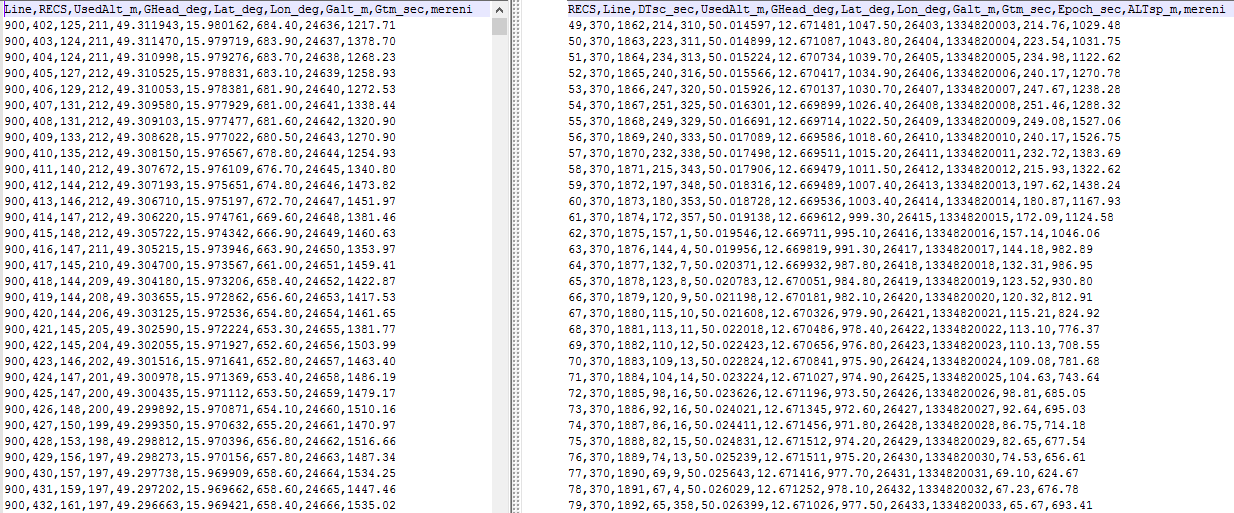
\includegraphics[scale=0.45]{./pictures/ukazka-vstup.png}
	\caption[Ukázka dvou typů vstupních souborů]{Ukázka dvou typů vstupních souborů
      \label{fig:ukazka-vstup}}
  \end{figure}

\section{Tělo zásuvného modulu}
\label{telo}

%%% ML: je opravdu Kosmogicky vhodne slovo s ohledem na vyznam teto vety?
Základ zásuvného modulu byl vytvořen ve volně šiřitelném mo\-dulu nazvaném Plugin
Builder\footnote{Dostupný na \textit{https://plugins.qgis.org/plugins/pluginbuilder/}}. Jedná se
%%% ML: napriklad ?
o~zásuvný modul vytvořený pro QGIS především (ale nikoli pouze) suitou kolem GeoApt LLC (například Gary
%%% ML: volne siritelny ?
Sherman), skupi\-ny zaměřující se na volně šiřitelný \zk{GIS}. Plugin Builder na
základě uživatelem zadaných parametrů vytvoří základní skelet zásuvného modulu - ikonku, holobyt
grafického rozhraní, metadata, základní funkce (zapnout, vypnout) a~vazby zásuvného modulu. 

Fundamentální tělo zajišťující základní funkcionalitu zásuvného modulu je ulože\-no v~několika vzájemně
provázaných souborech: 
\begin{itemize}

%%% ML: {\tt \_\_init\_\_.py} ?
	\item {\tt \_\_init\_\_.py}: Základní inicializace zásuvného modulu. 

	\item {\tt plugin\_upload.py}: Zajišťuje všeobecnou dostupnost zásuvného modulu. 	

	\item {\tt position\_correction.py}: Implementuje zásuvný modul do prostředí QGIS. Načítá jeho ikonu,
	jmenuje a~aktivuje jej a~v~případě vypínání se stará o~jeho destrukci. Funkce \textit{run} jej váže
	s~position\_correction\_dockwidget.py. 
	
	\item {\tt position\_correction\_dockwidget.py}: Nejdůle\-žitěj\-ší
	ze základních souborů zá\-suvného modulu. Volání
	souboru {\tt position\_correction\_dockwidget\_base.ui}
	vytvoře\-ného v~prostředí Qt Designer
	zde vyvolává grafické uživatelské rozhraní. Zajišťuje
	také funkčnost ve\-škerých jeho částí a~celkové
%%% ML: maat?
%%%%%% OP: maat je počeštěný, původem staroegyptský pojem, cosi jako bohatší řád - označuje celkově
%%%%%%     všeobecný řád, harmonii, správné fungování, zákonnost, stabilní jednání, kde se vše chová dle
%%%%%%     očekávání, jinak dojde ke kolapsu (počítačová řeč - erroru). Nahradím to chudším "řádem"
	dodržování vnitřního řádu, od načítání cest vstupních
	a~výstupních dat přes jejich zobrazování a~stylování (volá
%%% ML: provedeni posunu ?
	{\tt show\_as\_layer.py}) až po samotné provedení posunu ({\tt move.py}).
	Na pozadí dochází ke kontrole vstupujících údajů, v~případě nesrovnalostí
%%% ML: veta o nehodach a psovi mi prijde prilis sroubovana...
	bude uživatel u\-pozorněn chybovým hlášením. Aby se zamezilo zbrklým nehodám, byly ke zpřístupnění
	tlačítek zabudovány podmínky - ke zpřístupnění tlačítka na zobrazení vstupního souboru musí být
	k~tomuto souboru definována cesta, taktéž k~samotnému posunu je třeba mít vyplněny všechny potřebné
	parametry. 
	
	\item show\_as\_layer.py: Zobrazí soubor, an je předán jako jeden ze vstupních parame\-trů. Druhým
%%% ML: jako ze bych ty tridy implementoval sam od sebe, to nedava smysl
	vstupním parametrem je styl, jenž bude při zobrazování použit. Aby se zamezilo graviditě kódu
	a~obecné duplicitě kódu v~podhoubí prostředí QGIS, byly k~zobrazení využity interní objekty
	QgsVectorLayer a~QgsMapLayerRegistry. 

\end{itemize}

Toliko k~hrubému náčrtu fungování zásuvného modulu. Některé dílčí složky byly při představování
zane\-dbány, poněvadž nejsou k~pochopení fungování mo\-dulu nezbytné. Nyní se zvlášť podívejme na
soubory související se zkoumanou pro\-blematikou, tedy obsah move.py. 

%%% ML: krome pseudokodu (tam kde to pujde) doplnit obrazky
%%% zobrazujici danou situaci

\section{Posun o hodnoty}
\label{by_points}

%%% ML: by_points() je metoda tridy Move. + dalsi vyskyty
Posun o~hodnoty se skrývá pod metodou {\tt by\_points} třídy {\tt Move}.
Zde nejprve proběhne analýza vstupních dat.
Analýza spočívá v~prohledání hlavičky souboru, je třeba zjistit polohu hledaných hodnot - sloupce
{\tt Lat\_deg} a~{\tt Lon\_deg}. 

Následně se čte vstupní soubor řádek po řádku a~postup posunu se liší na základě vstupní hodnoty posunu. 

\subsection{Posun o kladný počet hodnot}
\label{kladnehodnoty}

%%% ML: doplnit pseudokod nebo diagram
Jedná-li se o~číslo kladné, připojujeme k~informacím bodu \textit{n} souřadnice bodu
\textit{n+x}, kde \textit{x} představuje hodnotu, o~niž body posouváme. Toho dosáhneme tím, že
%%% ML: preformulovat
v~každé smyčce cyklu postupně načteme \textit{x} řádků, přičemž první z~těchto řádků vložíme do proměnné
(zbylé se nikam neukládají a~v~paměti tak nezůstávají - zůstává vždy pouze poslední čtený);
v~paměti tedy zbude první a~poslední z~čtených řádků. Hodnoty ze sloupců souřadnic posledního
načteného řádku vložíme do příslušných sloupců prvního čteného řádku. Modifikovaný první
řádek se zapíše do výstupního souboru. Načte se poloha konce prvního řádku a~cyklus se může opakovat. 

    \begin{figure}[h]
    \centering
    \begin{algorithmic}[1]
    \STATE{posunovanyradek=přečti první řádek}
    \WHILE{existuje posunovanyradek}
    \STATE{pozice=ulož pozici ve vstupním souboru}
    \STATE{přečti \textit{x} řádků}
    \STATE{vlož souřadnice posledního čteného řádku do posunovanyradek}
    \STATE{zapiš posunovanyradek}
    \STATE{seek(pozice)}
    \STATE{posunovanyradek=přečti řádek}
    \ENDWHILE
    \end{algorithmic}
    \caption{Pseudokód - Posun o kladné hodnoty}
    \label{fig:pseudokladnehodnoty}
    \end{figure}

%%% ML: uvazit pridani pseudokodu i pro ostatni algoritmu
\subsection{Posun o záporný počet hodnot}
\label{zapornehodnoty}

Jedná-li se o~číslo záporné, ještě před cyklem se provede odečtení \textit{x}~řádků,
kde \textit{x} je hodnota posunu; tyto řádky jsou zapsány do seznamu hodnot.

Syžet cyklu následně probíhá
tím způsobem, že se z~tohoto seznamu odebírá první hodnota. Z~té jsou odečteny informace ze
sloupců příslušejících zeměpisným souřadnicím. Do dočasné proměnné je vložena poslední
hodnota seznamu a~její souřadnice jsou pře\-psány souřadnicemi výše zmiňovanými. Modifikovaný řádek
se zapíše do výstupního souboru. Nyní je třeba doplnit seznam opět na \textit{x} hodnot, toho
se dosáhne čtením dalšího řádku ze vstupního souboru a~jeho vložením na konec seznamu. Cyklus
se může opakovat. 

    \begin{figure}[h]
    \centering
    \begin{algorithmic}[1]
    \STATE{seznam=přečti \textit{x} řádků}
    \WHILE{existuje hodnota seznam[x]}
    \STATE{posunovanyradek=seznam[x]}
    \STATE{vlož souřadnice seznam[0] do posunovanyradek}
    \STATE{zapiš posunovanyradek}
    \STATE{vymaž seznam[0]}
    \STATE{seek(pozice)}
    \STATE{načti do seznamu další řádek}
    \ENDWHILE
    \end{algorithmic}
    \caption{Pseudokód - Posun o záporné hodnoty}
    \label{fig:pseudozapornehodnoty}
    \end{figure}

\subsection{Posun o nulový počet hodnot}
\label{nulovehodnoty}

Ve speciálním případě, kdy vstupuje do posunu o~hodnoty číslice~0,
dochází k~pouhé\-mu kopírování vstupního
souboru do souboru výstupního. Ovšem na žádný pád nemá v~takovém případě použití zásuvného modulu
odůvodnění. 

\section{Posun o konstantní vzdálenost}
\label{by_distance}

Posun o~konstantní vzdálenost je obsažen v~{\tt Move.by\_distance}. 

Na začátek funkce je třeba opět základní analýza vstupujícího souboru; její průběh je shodný
s~analýzou při posunu o~hodnoty. 

Následně je třeba připravit si pole pro výpočty na elipsoidu. Redundance kódu není v~ničím
zájmu, pro potřeby elipsoidických operací tedy užíváme knihovnu
prostředí QGIS {\tt QgsDistanceArea}. Zde nastavíme
užitý referenční elipsoid \zk{WGS84}. 

Výpočet se opět liší dle povahy vstupující hodnoty posunu (kladná vzdálenost,
záporná, 0). Posledním krokem před rozlišením, kterou větev výpočtu volání funkce vyvolá, je nastavení
%%% ML: chybi obecne provazanost v textu, zde napr. viz kapitola 2.y
parametrů elipsoidu pro výpočet první geodetické úlohy (ta v~{\tt QgsDistanceArea} implemetována
není, a~je třeba ji řešit v~samotném kódu). Pro její obecný popis viz
\ref{prvnigu}, kódové zpracování bude popsáno později v~\ref{prvniguplugin} 

\subsection{Posun o kladnou vzdálenost}
\label{kladnavzdalenost}

Posunujeme-li body o~kladnou vzdálenost, na první pohled se nezdá, že by se v~algoritmu skrývaly
nějaké záludnosti. Na pohled druhý ano. 

Nejzásadnější problém se vynoří, snaží-li se uživatel posunout body o~vzdálenost větší, než
jaká se rozpíná mezi dvěma body. V~takovém případě je třeba v~momentě překročení zmiňované
vzdálenosti přepočítat trajektorii na novou dvojici bodů a~o~tuto hodnotu požadovanou
délku posunu snížit. 

Z~tohoto důvodu proběhne v~každém cyklu čtení \textit{x} řádků ve vnořeném cyklu \textit{while}.
Tentokrát není \textit{x} daná hodnota, její velikost závisí na rozestupy mezi jednotlivými body.
V~každé smyčce vnitřního \textit{while} cyklu dojde k~výpočtu vzdálenosti mezi dvěma momentálně
načtenými body. Je-li vypočtená vzdálenost větší než délka posunu, cyklus skončí. 
Avšak není-li, délka posunu se zkrátí o~vzdálenost mezi těmito body a~bodem~2 se nahradí bod~1.
Vzápětí se čte další řádek představující nový bod~2 a~cyklus se opakuje. V~momentě, kdy
skončí, máme tedy novou dvojici bodů a~zbytek z posunu náležející na tento úsek.
%%% ML: probiha? poli?
Výpočet první geodetické úlohy tedy probíhá až v~takto předpřipraveném prostředí. 

Kromě zeměpisných souřadnic je ale třeba veškeré ostatní informace převzít z~prvního
čteného řádku (jediný, který kromě momentálního páru bodů zůstává v~paměti). Takto vytvořený
řádek se zapíše do výstupního souboru. Načte se poloha konce prvního čteného řádku
a~vnější cyklus se může opakovat. 

\subsection{Posun o zápornou vzdálenost}
\label{zapornavzdalenost}

Vstupuje-li do posunu o~konstantní vzdálenost záporná hodnota, nabízí se možnost
využití kódu pro kladnou hodnotu, pouze s~inversně vyměněnými body. Opět bychom ale narazili
ve chvíli, kdy posun překračuje vzdálenost mezi dvěma body. 

Zde je zapotřebí jiného způsobu řešení problému. Tento úkol ztěžuje ještě fakt, že nechceme
zahltit paměť načítáním celého vstupního souboru, snažíme se tedy pracovat jen s~nutně
potřebnou dávkou řádků. 

Opět si vypomůžeme seznamem hodnot (řádků). Ponejprve byl vytvořen vstup\-ní seznam
na stejném principu, jako v~předchozím případě (porovnávání \textit{uražené} vzdálenosti se
vzdáleností mezi body), s~tím rozdílem, že tentokráte již použité body vkládáme do seznamu hodnot.

Základní cyklus, jenž by se poznovu dal nazvat cyklem vnějším, se skládá ze dvou na sebe
navazujících cyklů vnitřních. 

První vnitřní cyklus slouží k revizi, zda není seznam vstupující do výpočtu zbytečně obsáhlý.
Zjistí-li, že posun nepřekročí více než \textit{x} prvků, smaže redundantní prvky z~počátku seznamu (posouváme bod
z~konce seznamu). Na každý pád vstupuje do výpočtu seznam o~rozsahu právě onoho \textit{x}. 

Po dobrozdání výpočet vstupuje do cyklu spočívajícího ve výpočtu první geode\-tické úlohy.
Nadto do tohoto cyklu vstupují hodnoty kvůli posunu zpět v~reversním pořádku. Měl-li by
posun překročit vzdálenost mezi dvěma body, kvůli úspoře se výpočet přeskočí a~do pomocných
proměnných se zapíšou přímo souřadnice druhého z~bodů. 

Po smyčce, při kteréž již dojde k~výpočtu první geodetické úlohy, je proveden zápis do výstupního
souboru - zapíše se poslední řádek ze seznamu se zeměpisnými souřadnicemi přepsanými
souřadnicemi vypočtenými. 

\subsection{Posun o nulovou vzdálenost}
\label{nulovavzdalenost}

Ježto by měl zásuvný modul fungovat i~při
operacích, které kterakkolivěk postrádají důvod k~jeho využití, byl do jeho
vnitřností implementován i~posun o~nulovou vzdálenost.
V~takovém případě se však vážně nejedná o~posun, nýbrž o~pouhé přepsání
neupravených hodnot ze vstupního souboru do souboru výstupního. 

\subsection{První geodetická úloha}
\label{prvniguplugin}

%%% ML: tady uz odkaz na teoretickou cast je, to je v poradku, v dalsim textu casto chybi
Velký problém při výpočtech na elipsoidu představuje první geodetická úloha. Ta byla popsána
již výše v~kapitole \ref{prvnigu}, nyní tedy pouze několiko poznámek k~jejímu kódovému zpracování. 

Samotný kód posunů se pro své značné množství nutných podmínek a~cyklů nevyznačuje
elegantní přehledností, pročež byl alespoň výpočet první geodetické úlohy vytržen jako zvláštní funkce.

Výpočet probíhá na základě iterací. Anžto byl jejich postup již výše popsán, jen zdůrazníme
některé části. Každá z~iterací zpřesňuje výpočet a~tyto iterace jsou prováděny do doby,
kdy přesnost dosáhne 0.0000000001~radiánu. 

Důležitým prvkem, který by neměl zůstat opomenut, jest vstupující azimut. Zde se musí pamatovat
na to, že azimut na elipsoidu se od azimutu na kouli či v~ro\-vině liší. Z~tohoto
důvodu byla využita funkce {\tt computeDistanceBearing} knihovny {\tt QgsDistanceArea}.

Nyní by bylo vhodné zdůvodnit právě tento druh výpočtu první geodetické úlohy a~nepoužití
složitější, arciť přesnější metody interpolace. 

Chtěli-li bychom vytvořit kód, který vykresluje trajektorii pravděpodobněji, mu\-sel by do
výpočtu vstupovat kompletní vstupní soubor; a~vzhledem k~tomu, že není ničím neobvyklým
soubor čítající mnoho přes 10000 záznamů o více než desítce sloupců, rozdíl v~systémové zátěži
by byl obrovský. 

Přesto byl tento návrh zpraco\-vá\-ní na poradě se Státním ústavem radiační ochra\-ny
vznesen. Po projednání bylo ze strany \zk{SÚRO} uvedeno, že vyhovuje námi momentálně
používaný způsob výpočtu; a~to nikolivěk pouze z~důvodu úspory systémových nároků, nýbrž především
z~toho důvodu, že výsledné zpřesnění souřadnic už by mělo na výsledky jejich práce
prakticky nulový vliv. 

\section{Posun o konstantní čas (proměnnou vzdálenost)}
\label{by_seconds}

Velká část popisu kódu v~kapitole \ref{by_distance} se týká též posunu o~konstantní
čas - o~vzdále\-nost s~uvážením rychlosti. Odkazujeme se zde na základní přípravu hrací plochy,
analýzu, parametry elipsoidu a~vyvolání knihovny {\tt QgsDistanceArea}. Též výpočet první geodetické
úlohy se shoduje s výše popsanými postupy. Co se problémů jednotlivých
segmentů týče, dá se říci, že se dědí problémy posunu o~konstantní vzdálenost, pouze se k~nim
přidávají některé nové. 

Též základní fungování částí funkce se od těch popsaných výše příliš neliší; po\-psány tedy
budou pouze případné zásadnější odlišnosti. 

Nejočividnější rozdíl je pro veškeré posuny o~čas stejný - výpočet vzdálenosti,
o~niž se bod posouvá. Nejdříve je zapotřebí funkcí {\tt computeDistanceBearing}
vypočítat vzdálenost mezi dvojicí bodů. Vydělíme-li ji časovým úsekem, za který tuto vzdálenost
měřicí zařízení urazilo, získáme momentální rychlost. K~požadované délce posunu
se dostaneme již pouhým vynásobením této rychlosti uživatelem zadaným časovým úsekem. 

Z~uvedeného vyplývá, že je mezi dvojicí bodů předpokládán lineární pohyb. Taková idea vzešla
již od Státního ústavu radiační ochrany na základě toho, že vrtulník začíná měřit
až po jisté uražené vzdálenosti. V~tomto momentě již nabyl rychlost, kterou se snaží během
celého procesu měření konstantně udržovat. 

Zásadním problémem, který se při zpracování vynořil, je nejednotnost měření.
Ačkolivěk bývá zvykem měřit data po jedné sekundě, nedá se na takový postup spoléhat.
Používal-li by zásuvný modul cizinec, není vyloučené, že by v~jeho zemi bylo územ měřit
data po vteřinách třech nebo pěti. Je tedy třeba pracovat s~časovými značkami ze sloupce
{\tt Gtm\_sec} a~jejich rozdíly. Tím dochází k~zesložitění kódu, ale rovněž k~potřebnému
podchycení případných nesrovnalostí. 

Též je třeba ověřovat body vstupující do výpočtu první geodetické úlohy. Má-li měřicí zařízení
omezenou přesnost, může se stát, že budou mít dva po sobě měřené body zapsány stejné souřadnice.
Pokud by k~takové situaci došlo, je třeba se vyhnout výpočtu geodetické úlohy. Problém ani
tak nespočívá v~azimutu, jenž by mohl nabývat jakékoli hodnoty, nýbrž ve vzdálenosti.
Dělení nulou by vyvolávalo ve výpočtech chybu. Anžto vzdálenost mezi body jest nulová,
nastane zápis souřadnic jednoho z~bodů. 

\subsection{Posun o kladný časový úsek}
\label{kladnycas}

Při posunu o~kladný časový úsek je třeba vytvořit si pomocnou proměnnou, nazvěme ji zde \textit{x},
představující čas, o~který momentální bod posouváme. Ve chvíli vytvoření tedy bude \textit{x}
rovno uživatelem zadané hodnotě posunu. 

Před základním cyklem dojde k~odečtení a~uložení prvního řádku. Ten představuje posouvaný bod.
V~základním cyklu pak algoritmus čte další řádek. Ten představuje bod, k~němuž směřuje
trajektorie, po níž prvý bod posouváme. 

V~tomto vnějším cyklu opět pracuje cyklus vnitřní, v~kterémžto dochází k~porov\-ná\-vá\-ní našeho
\textit{x} s~dobou, za kterou měřicí zařízení urazilo vzdálenost mezi právě načtenou dvojicí bodů. 

Je-li \textit{x} menší než tato doba, proběhne výpočet první geodetické úlohy na trajektorii
a~s~uvážením rychlosti mezi těmito dvěma body. 

Pokud se tyto hodnoty rovnají, jedná se o~podmínky pro výpočet ještě příznivější. Dojde k~pouhému
zápisu souřadnic druhého bodu do příslušných proměnných. V~ta\-ko\-vém
případě by se posun dal označit za posun o~hodnoty. 

Zákeřněji působí možnost, při níž je hodnota \textit{x} větší než doba mezi měřením dvou
bodů v~momentální paměti. Pak je zapotřebí dobu posunu \textit{x} zmenšit o~dobu, kterou
vrtulník mezi dvěma body urazil, druhý bod vložit do bodu prvního a~načíst nový druhý bod. Následně
se vnitřní cyklus zabývající se dobrozdáním ohledně hodnoty \textit{x} a~hodnoty
rozdílu časových značek mezi dvěma body v~paměti může opakovat. 

Poté, co jednou z~možných cest skončí vnitřní cyklus, dojde k~vložení nových souřadnic
(ať už vypočtených, nebo jen vyjmutých) do odpovídajících sloupců první\-ho čteného řádku.
Ten se zapíše do výstupního souboru, do proměnné \textit{x} se opět načte uživatelem volená
hodnota posunu, ve čtení se vyvolá pozice před započetím vnitřního cyklu, a~vnější cyklus se
opakuje s~řádky o~jeden posunutými. 

\subsection{Posun o záporný časový úsek}
\label{zapornycas}

Pro posun o~záporný časový úsek se jako ideální řešení opět zdálo využití seznamu řádků.
Tento seznam byl načten před samotným započetím vnějšího cyklu a~hodnoty do něj byly
přidávány do té doby, dokud součet rozdílů časových značek mezi jednotlivými body
nepřekročí uživatelem požadovanou hodnotu posunu (lépe řečeno její absolutní hodnotu,
poněvadž uživatel volí hodnotu zápornou). 

Seznam již vstupuje do vnějšího cyklu, jehož cílem je postupně projít celý vstupní
soubor a~posunout veškeré body. Tento cyklus se skládá ze dvou cyklů vnitřních. 

První vnitřní cyklus reviduje vstupující seznam hodnot. Zjišťuje, zda není přes\-příliš obsáhlý.
Kontrolu provádí na základě porovnávání součtu rozdílů časových značek s~uživatelem
voleným časovým posunem. Narazí-li algoritmus na hodnoty, jež by nebyly při výpočtu využity,
ze seznamu je kvůli úspoře paměti umaže (protože se nové hodnoty - posouvající se body - přidávají
na konec seznamu, nadbytečné hodnoty se nachází na jeho začátku). Tyto řádky totiž nebudou
třeba ani k~žádné z~následujících smyček. 

Druhý z~vnitřních cyklů se příliš neliší od toho popsaného v~kapitole \ref{zapornavzdalenost}.
Čte v~reversním pořadí seznam hodnot a~spočívá v~analýze vstupujících dat. Analýza
probíhá s~pomocnou proměnnou (ze zvyku si ji označme
\textit{x}), která představuje čas posunu od momentálního bodu. 

Pokud \textit{x} převyšuje dobu, za niž měřicí zařízení urazilo vzdálenost mezi dvěma načtenými
body, pouze se posuneme v~seznamu o úroveň níže (bod~1 se stane bodem 2 a~do nového
bodu 1 se vloží další řádek seznamu); \textit{x} se zmenší o~velikost zmiňovaného časového úseku. 

Rovnají-li se tyto dvě hodnoty, do paměti se uloží
souřadnice bodu 1 (bodu, k~němuž se počítá trajektorie). 

V~případě, že je absolutní hodnota \textit{x} menší než rozdíl časových značek, dochází
k~výpočtu první geodetické úlohy. 

Následuje chvíle pro již typickou koncovku vnějšího cyklu. Souřadnice z~paměti se vloží
do odpovídajících sloupců řádku s~posunovaným bodem a~ten se zapíše do výstupního souboru.
Následně se na konec seznamu hodnot načte další řádek (nový posunovaný bod) a~\textit{x}
se nastaví na uživatelem volenou hodnotu posunu. Cyklus pokračuje další smyčkou. 

\subsection{Posun o nulový časový úsek}
\label{nulovycas}

Byť živou věcí neexistuje důvod k~použití zásuvného modulu za účelem takové ope\-race,
dovede si zásuvný modul poradit i~s~případem posunu o~0~sekund. Abychom se vyhnuli
naprosto zbytečné zátěži ve formě počítání nulových posunů, poznovu tato část kódu
funguje jen jako kopírování vstupního souboru do souboru výstupního. 

\section{Licence}
\label{licence}

Nebtě byl zásuvný modul vytvořen pro QGIS a~využívá jeho knihoven, dědí jeho licenci: GNU General Public
License~(\zk{GPL}). 

Jde o~\textit{copyleftovou} (odvozené dílo musí být dostupné pod stejnou licencí)
licenci. Ve své podstatě zde nejde o~omezování svobody, alebrž právě o~její dodržování - zajišťuje,
aby prvotně svobodný software tuto svobodu modifikacemi či přidáváním neztratil. 




\chapter{Závěr}
\label{zaver}

Cílem této bakalářské práce byla tvorba
softwarového nástroje umožňujícího posun letecky
měřených bodů po trajektorii a~jeho implementace
do prostředí QGIS jako tzv.~zásuvného modulu. 

Celý projekt se zakládal na pracích Státního
ústavu radiační ochrany (\zk{SÚRO}). Ten dosud prováděl posun
tak, že každému bodu pouze přiřadil souřadnice bodu
předcházejícího či následujícího (s~libovolným
krokem). Přihlédneme-li k~bouchoři, kterým podobný posun
o~hodnoty jest, můžeme říci, že bylo zadání
nejen splněno, ale na základě návrhů \zk{SÚRO}
dovedeno ještě dále. 

V~současnosti zásuvný modul umožňuje posun dat
nikoli jen o~hodnoty, nýbrž také o~konstantní
vzdálenost či o~čas (tj.~o~vzdálenost
s~uvážením rychlosti). V~grafic\-kém
rozhraní si může uživatel též zvolit styl,
který by chtěl pro zobrazení vstupních
a~výstupních dat použít. 

V~čase budoucím se nabízejí některá rozšíření
stávající funkcionality. Počítá se s~implementací
více stylů běžně užívaných při zpracování. Bylo by
rovněž vhodné dát uživateli možnost zvolit
referenční elipsoid ad libitum; momentálně
probíhají veš\-keré výpočty na elipsoidu \zk{WGS84}.
Veškerá dostupná data sice obsahují zeměpisné souřadnice
právě na tomto elipsoidu, nelze ale vyloučit, že
se v~cizině vyskytují i~nějaké adventivní případy.

%%% ML: zde by se hodil odkaz na xml soubor QGIS repozitare
Zásuvný modul byl pod hlavičkou \textit{experimentální}
\href{http://geo.fsv.cvut.cz/osgeorel/qgis-plugins.xml}{uveřejněn} a~v~\zk{SÚRO} již od dubna~2016 probíhají testy.




% Vysázení seznamu zkratek

\begin{seznamzkratek}{ABCDE}

	\novazkratka{SÚRO}
	      {SÚRO}
	      {Státní ústav radiační ochrany}
	      
	\novazkratka{PSF}
		  {PSF}
	      {Python Software Foundation}

	\novazkratka{GIS}
	      {GIS}
	      {Geografický informační systém}

      \novazkratka{OSGeo}
	      {OSGeo}
	      {Open Source Geospatial Foundation}

      \novazkratka{SQL}	
	      {SQL}
	      {Structured Query Language}
	      
	  \novazkratka{GUI}	
	      {GUI}
	      {Grafické uživatelské rozhraní (Graphical user interface)}
	      
	  \novazkratka{CSV}	
	      {CSV}
	      {Hodnoty oddělené čárkami (Comma-separated values)}
	      
	  \novazkratka{WGS84}	
	      {WGS84}
	      {Světový geodetický systém 1984 (World Geodetic System 1984)}

	  \novazkratka{GPL}	
	      {GPL}
	      {Všeobecná veřejná licence (General Public License)}

\end{seznamzkratek}

% Literatura
\nocite{*}
\def\refname{Literatura}
\bibliographystyle{mystyle}
\bibliography{literatura}


% Začátek příloh
\prilohy

% Vysázení seznamu příloh
\seznampriloh

% Vložení souboru s přílohami


%%%%%%%%%%%%%%%%%%%%%%%%%%%%%%%%%%%%%%%%%%%%%%%%%%%%%%%%%%%%%%%%%%%%%%%%%%%%%%%%%%%
%%                 PŘÍLOHA - UŽIVATELSKÁ PŘÍRUČKA                                %%
%%%%%%%%%%%%%%%%%%%%%%%%%%%%%%%%%%%%%%%%%%%%%%%%%%%%%%%%%%%%%%%%%%%%%%%%%%%%%%%%%%%
\chapter{User guide}
\label{user-guide}

This user guide is written for plugin using in QGIS 2.12. There is a~possibility that works with plugin
will be different in other versions of QGIS. 

\section{Loading of plugin}
\label{plugin-load}

* 
* 

* 
* TUHLE ČÁST JEŠTĚ MUSÍM DOPSAT - NEJDŘÍV JE POTŘEBA PLUGIN ZE SLOŽKY SUROLEVELING FUNKČNĚ PŘESUNOUT DO GPS POSITION LAG CORRECTION, ABYCH VĚDĚL, JAK SE BUDE V NABÍDCE PLUGIN JMENOVAT
*

* 
*

\section{Work with plugin}
\label{work}

In this section will be described primary functions and working of graphical user interface of plugin. 

  \begin{figure}[H]
   \centering
	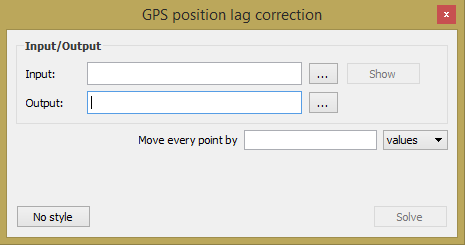
\includegraphics[scale=0.75]{./pictures/gui.png}
	\caption[GUI]{GUI}
      \label{fig:gui}
  \end{figure}

\subsection{Input and output defining}
\label{input-output}

The basic elements are of course input and output. 

In input, you have to define the~file you want to work with. You can write the~path to this file or
there is the~button with {\tt ...}. If you click on this button, you will get the~interface where
you can choose the~path to your file. Click on OK will insert this path to lineedit in basic GUI. Click
on Cancel will interrupt the~interface for choose, and the~content of lineedit will not be changed. 

  \begin{figure}[H]
   \centering
	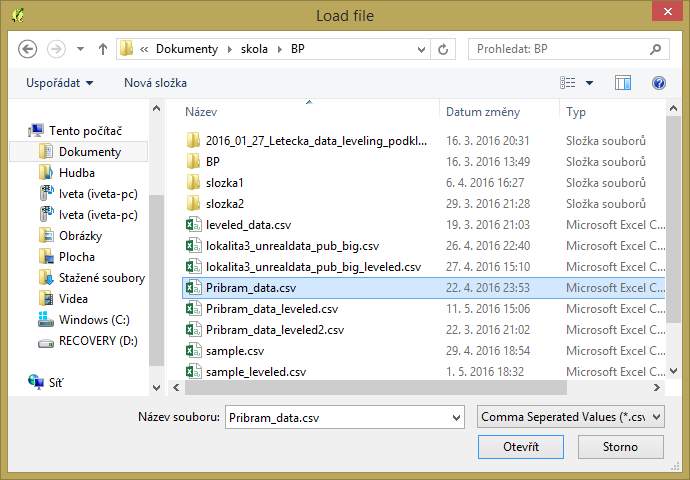
\includegraphics[scale=0.75]{./pictures/input.png}
	\caption[Loading input]{Loading input}
      \label{fig:input}
  \end{figure}

The~same work is with output, but there you define the~path where the~new file will be created.
You can manually define the~path or use the~browse button. You will again get a~new interface, this
time created for choosing folder. 

  \begin{figure}[H]
   \centering
	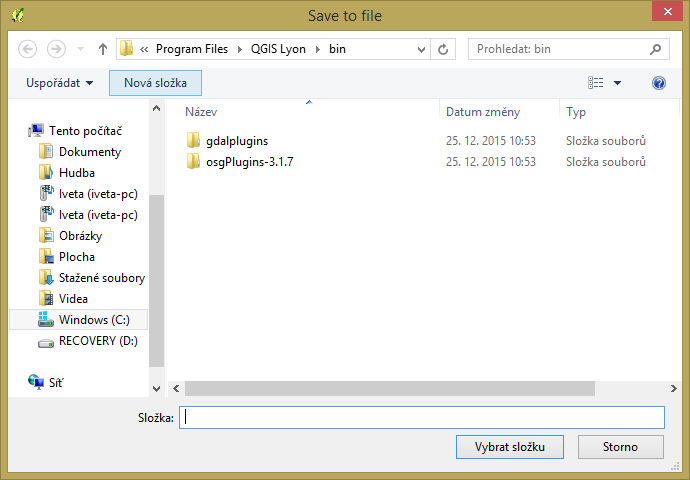
\includegraphics[scale=0.75]{./pictures/output.png}
	\caption[Choosing output directory]{Choosing output directory}
      \label{fig:output}
  \end{figure}

\subsection{Styling}
\label{styling}

There is also additional possibility of styling your points for better visualisation. 

In the~default GUI is the~button \textit{No style}. It means that you have not defined any style
and points will be created in default QGIS style. If you want your own style, you have to click on
this button. You will get the~browsing interface. You are automatically directed to folder
\textit{styles} in the~plugin folder; you have to choose qml file and click OK. Click on Cancel will
interrupt the interface and set again \textit{No style}. 

  \begin{figure}[H]
   \centering
	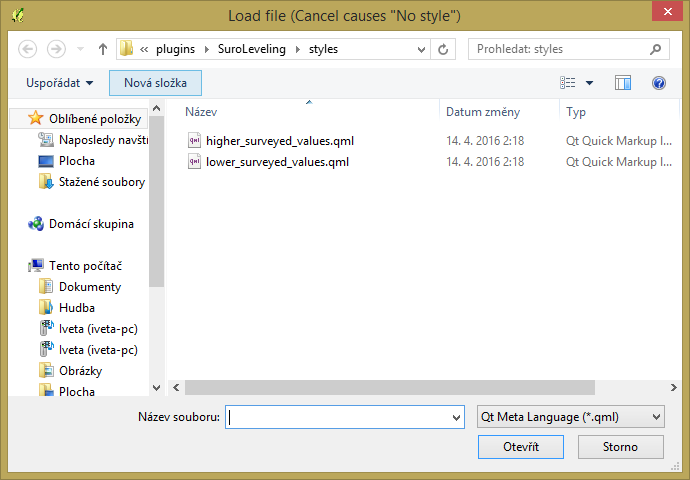
\includegraphics[scale=0.75]{./pictures/style.png}
	\caption[Choose style]{Choose style}
      \label{fig:style}
  \end{figure}

If you have chosen your own style, you would see its name on the~style button. 

  \begin{figure}[H]
   \centering
	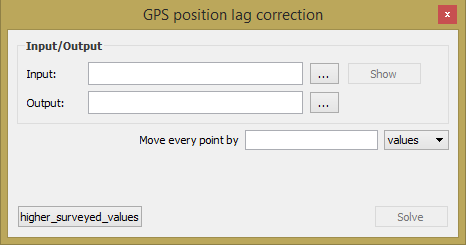
\includegraphics[scale=0.75]{./pictures/style-defined.png}
	\caption[Used style]{Used style}
      \label{fig:used-style}
  \end{figure}

In the~default version of plugin there are two default styles. Styling in those styles is based on
column mereni – one style for higher and one style for lower values. 

\subsection{Showing input}
\label{show}

Next to input is the button \textit{Show}. 

Show button is just to visualise the input file as layer in QGIS. It has no effect on the run of plugin
and it is not necessary for the~run, but it allows you to visualise the~input file in the same style as
the~output file. It gives you also the~opportunity to compare the~moved values with the~original ones. 

This button was created on request by users who prefer to visualise both the~input and the~output in
the~same interface. 

If input file does not exists, plugin will raise the~error message. 

\subsection{Move}
\label{move}

Move will be done by clicking on button \textit{Solve}. Before moving you have to define few more things. 

In combobox you can choose the~units of move – each presents other type of move; values mean move
by values, meters mean move by constant distance and seconds mean move by constant time/variable
distance considering current velocity. 

In the~appropriate lineedit you have to insert value of move. For values it should be integer (it
does not make sense to move point by 1.5 values because nothing like 1.5 value does not exist), for
other moves it should be integer or float. 

For wrong input, plugin will raise the~error message. 

\subsection{Dependencies}
\label{dependencies}

To avoid some unnecessary errors, there are some dependencies in the~plugin GUI. 

The~first is \textit{Show} button. This button is
disabled until you have wrote anything into input lineedit. 

  \begin{figure}[H]
   \centering
	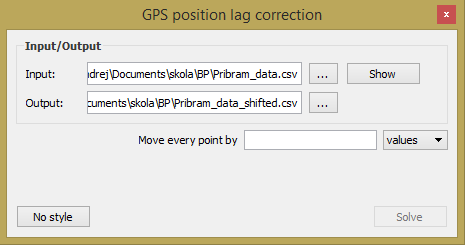
\includegraphics[scale=0.75]{./pictures/show.png}
	\caption[Enabled Show button]{Enabled Show button}
      \label{fig:show}
  \end{figure}

The~second is button \textit{Solve}. You can’t solve anything until you have defined input, output and
value of move.

  \begin{figure}[H]
   \centering
	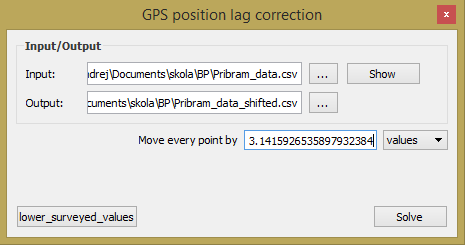
\includegraphics[scale=0.75]{./pictures/solve.png}
	\caption[Enabled Solve button]{Enabled Solve button}
      \label{fig:solve}
  \end{figure}

There is also implemented shortcut for defining output directory. Many users wants to save output file to
the~directory from which was read the~input file, so when you choose input file, the~directory will
be automatically copied into output lineedit, just with added \textit{\_moved} into filename. 


% Konec dokumentu
\end{document}
